\chapter{硅波导和混合集成III-V波导的模式耦合}
\section{背景介绍}
硅基混合集成III-V平台光器件的一个共性问题就是混合集成III-V波导和硅波导模式的耦合。硅波导和硅基混合集成III-V波导的模式如图\ref{fig_ch3_si_hybrid_mode}所示,在能量分布和等效折射率上都有很大的差别。目前,采用的方案是利用锥形(taper)结构。在硅波导的锥形结构上,宽度逐渐减小,而对应的III-V波导上宽度则逐渐增大,从而使硅波导上的光缓慢耦合到III-V波导中。图\ref{fig_ch3_background_str}(a, b)展示了目前采用的用于硅波导和混合集成III-V波导的多层或者多段锥形耦合结构\cite{kurczveil2013characterization, keyvaninia2009engineering}。这些耦合结构的尺寸都在40 ~$\mu m$以上,被广泛用于混合集成的激光器,探测器和调制器。由于光器件的小型化,能增加光器件的集成度,降低单个光器件的成本,所以目前硅基光子器件的一个趋势是将原先的器件的尺寸缩小。为此,文献[\citenum{wang2012heterogeneous}]将线性锥形结构变为曲形锥形结构,如图\ref{fig_ch3_background_str}(c)所示,将耦合结构尺寸缩小到了$25~\mu m$。不过,并没说明耦合结构是否还可以进一步减小。
\begin{figure}[htb]
	\small
	\subfigure[]{
		\begin{minipage}[]{0.5\textwidth}
			\centering
			\label{fig_ch3_si_mode}
			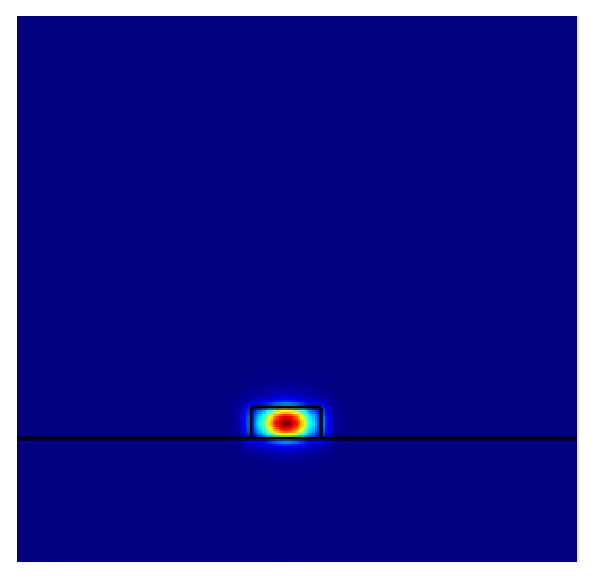
\includegraphics[width=6cm]{./Pictures/fig_ch3_si_mode.eps}
		\end{minipage}}
	\subfigure[]{
		\begin{minipage}[]{0.5\textwidth}
			\centering
			\label{fig_ch3_hybrid_mode} %% label for second subfigure
			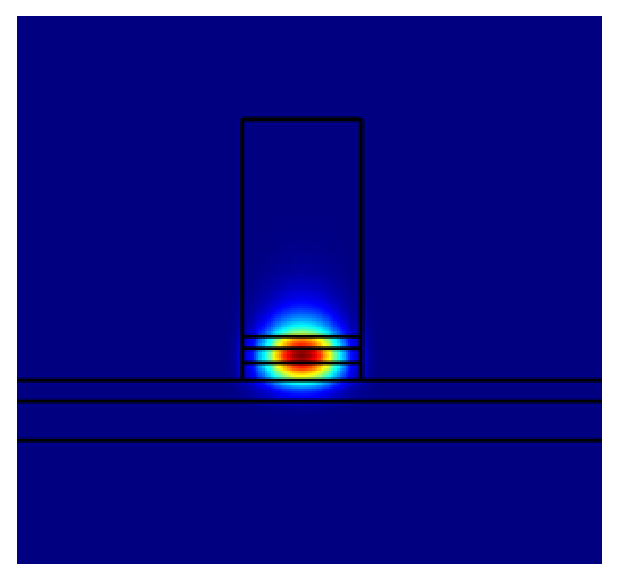
\includegraphics[width=6cm]{./Pictures/fig_ch3_hybrid_mode.eps}
		\end{minipage}}
	\caption{(a)$600~nm$宽硅波导的模式,其等效折射率$n_{eff}=2.58$;(b)$1~\mu m$宽硅基混合集成III-V波导的模式,其等效折射率$n_{eff}=3.19$}
	\label{fig_ch3_si_hybrid_mode}	
\end{figure}
		
\begin{figure}[htb]
	\centering
	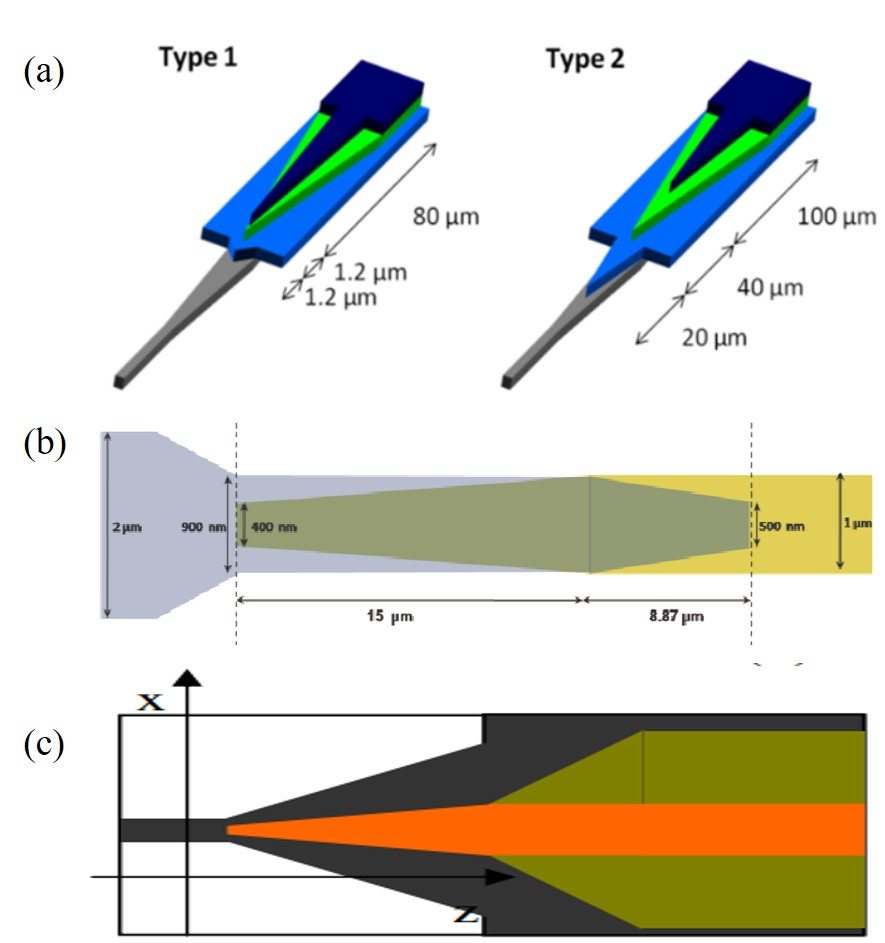
\includegraphics[width=12cm]{./Pictures/fig_ch3_background_str.jpg}
	\caption{ 目前硅波导和混合集成III-V波导的模式耦合结构(a) 多层锥形耦合结构\cite{kurczveil2013characterization};(b)多段锥形耦合结构\cite{keyvaninia2009engineering};(c)曲形锥形结构\cite{wang2012heterogeneous}}
	\label{fig_ch3_background_str}
\end{figure}

我们在尝试减小耦合尺寸时,首次发现限制耦合长度的重要因素是来自于III-V波导的高阶模式,我们通过设计三段式耦合结构,充分利用III-V材料选择性刻蚀的特点,形成近似三维锥形结构,将光缓慢地从硅波导耦合到III-V波导中。通过这种方法我们设计了长度只有8~$\mu m$的导耦合结构。这个结构能实现了95\%以上的能量耦合,并且相应带宽也能达到100 nm。随后我们探索了用电子书光刻(Electron Beam Lithography, E-Beam)制作这种紧凑耦合结构的工艺流程。
\section{紧凑型三段式耦合结构的设计}
为了验证这种紧凑型三段式耦合结构的设计方法,我们采用的III-V材料厚度和折射率如表\ref{IIIV_qian_str}与文献[\citenum{wang2012heterogeneous}]相同。这样也便于比较我们的设计思路。硅基混合集成III-V波导的截面示意图如图\ref{fig_ch3_3d_taper}(a)所示。硅波导的上表面和III-V的下表面我们定义为键合层的厚度为$h_{BCB}$。
{
	\begin{table}[htb]
		\zihao{5}
		\caption{III-V材料各层的厚度和折射率}
		\label{IIIV_qian_str}
		\centering
		\begin{tabular}[t]{lll}
			\hline
			名称  & 厚度~$(\mu m)$  & 折射率 \\
			\hline
			DVS-BCB & - & 1.543\\
			p-cladding & 1.5 &3.17 \\
			SCH & 0.08 & 3.46 \\
			MQW & 0.1 & 3.52 \\
			SCH & 0.12 & 3.46 \\
			n-contact & 0.14 & 3.17 \\
			Si & 0.22 & 3.477 \\
			SiO2 & 1 & 1.45 \\
			\hline
		\end{tabular}
	\end{table}
}

\begin{figure}[htb]
	\centering
	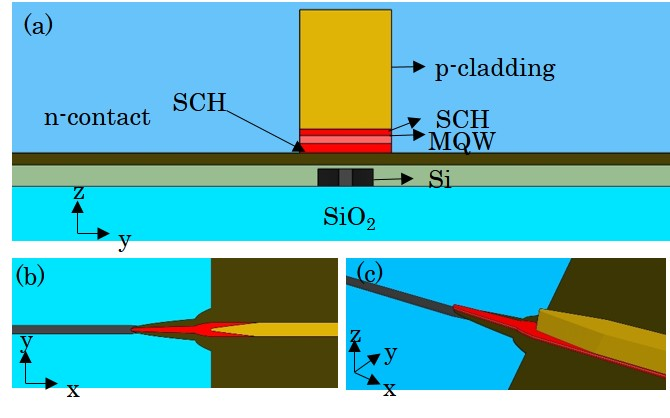
\includegraphics[width=12cm]{./Pictures/fig_ch3_3d_taper.jpg}
	\caption{紧凑型三段锥形耦合器的结构图:(a) 波导剖面图;(b)俯视图;(c)三维立体视图}
	\label{fig_ch3_3d_taper}
\end{figure}


图\ref{fig_ch3_3d_taper}(b)和\ref{fig_ch3_3d_taper}(c)展示了所提出的锥形耦合结构的示意图。从图中可以看出了,锥形耦合结构分成了三段结构。在第一段结构中,光从硅波导首先耦合到0.44~$\mu m$厚的由两个SCH层,MQW层和n-contact层构成的III-V波导中。在第二段结构中,0.44~$\mu m$厚的III-V波导的宽度逐渐增加,提高光在MQW层的限制能力。在第二段结构的末尾光的模场已经和最终所需的模式几乎相匹配。因此在第三段结构,我们可以将最厚的p-cladding层通过一个很短的锥形结构引入。通过三段式的锥形耦合结构,可以将整个模式耦合的长度大大缩短。

两根垂直分离的波导中两个模式相互耦合的问题已经在文献[\citenum{sun2009adiabaticity}]中进行详细的理论分析,并且给出了最短耦合长度的解析解。当两根分立波导的模式所对应的等效折射率随波导的长度有相交,并且两个光场模式的对称性相同时,那么两个波导靠近,就会有光模式的相互耦合。然而,文献[\citenum{sun2009adiabaticity}]的理论中,仅考虑了每根波导只有基模的情况。然而,实际中III-V波导,却拥有很多高阶模式。如果在耦合结构中,这些高阶模式的等效折射率变化也和硅波导的等效折射率变化有所相交,那么硅波导的部分光能量就会耦合到III-V波导的高阶模式中去。

图\ref{fig_ch3_multimode}(a)展示了,当p-cladding存在时的传统III-V波导模式的等效折射率$(n_{eff})$随波导宽度变化的关系。我们可以看到此时III-V支持很多高阶模式,并且高阶模式和基模之间的等效折射率差很小。另外一方面,从图\ref{fig_ch3_multimode}(b),我们可以看到当III-V波导没有很厚的p-cladding时,III-V波导只支持相对较少的模式。此时高阶模式和基模等效折射率的差距,见图\ref{fig_ch3_multimode}(b),也比之前有所提高。这意味着,在硅波导的基模转化成III-V波导的基模时,III-V波导高阶模式的影响就明显减弱。因此,利用没有p-cladding层的III-V波导,可以实现硅和III-V之间紧凑的耦合结构。这种三段式锥形结构不仅拥有多层锥形耦合结构少反射率的特点\cite{kurczveil2013characterization},也利用第一段的没有p-cladding III-V锥形波导阻止了高阶模式的产生。通过将整个锥形耦合结构分成独立的三段,我们可以对每段锥形耦合结构单独的优化。接下来,我们就讨论每段taper的优化过程。

\begin{figure}[htb]
	\centering
	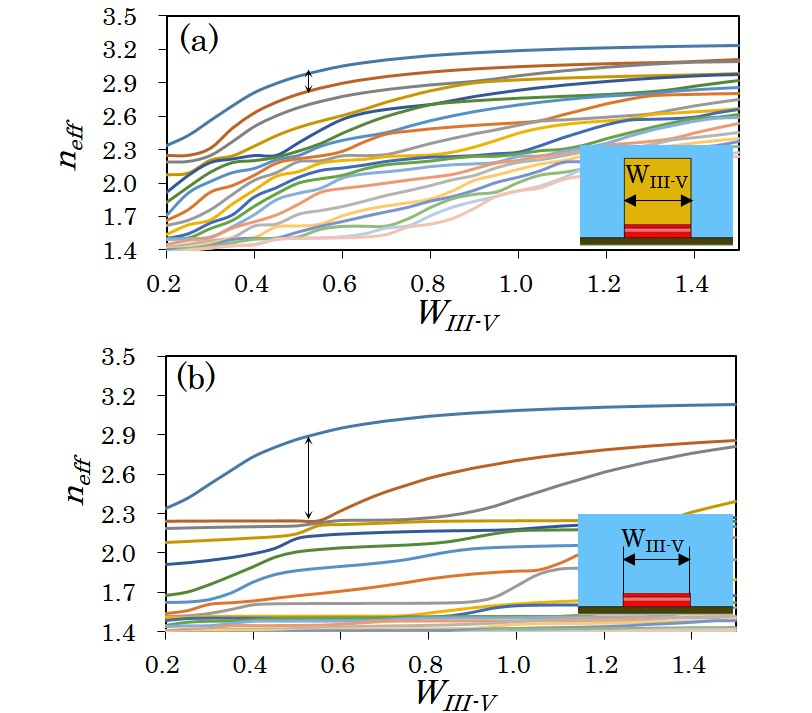
\includegraphics[width=12cm]{./Pictures/fig_ch3_multimode.jpg}
	\caption{模式等效折射率$n_{eff}$随着III-V波导宽度的变化:(a) III-V波导包含p-cladding层;(b)III-V波导没有p-cladding层}
	\label{fig_ch3_multimode}
\end{figure}

三段式的锥形耦合结构可以通过选择性湿法腐蚀的工艺制作,这个方法也被用于制作多层锥形结构\cite{kurczveil2013characterization}。图\ref{fig_ch3_detail_structure}展示了详细的设计结构参数。所有锥形结构的尖端宽度$(W_{tip})$受到工艺的限制。更细小的尖端意味着更小的反射。在此,我们同文献[\citenum{wang2012heterogeneous}]相同,$W_{tip} = 0.15~\mu m$。输入硅波导的宽度是$0.6~\mu m$。在第三段锥形结构中,最后的硅基混合集成III-V波导的MQW层的宽度$W_{mqw2}$与p-cladding的宽度$W_{pInP}$相同,我们在此选取$W_{mqw2}$为最后波导的宽度。$W_{mqw2}$是通过优化光的约束因子来确定。图\ref{fig_ch3_confinement}展示了在$W_{mqw2}$变化时,100 nm厚的MQW层对光的约束因子。我们可以看到当$W_{mqw2} > 0.5~\mu m$时,光的限制因子已经趋于稳定。在此,我们选取$W_{mqw2} = 1 ~\mu m$,此时,光限制因子已经达到25\%的稳定值。

\begin{figure}[htb]
	\centering
	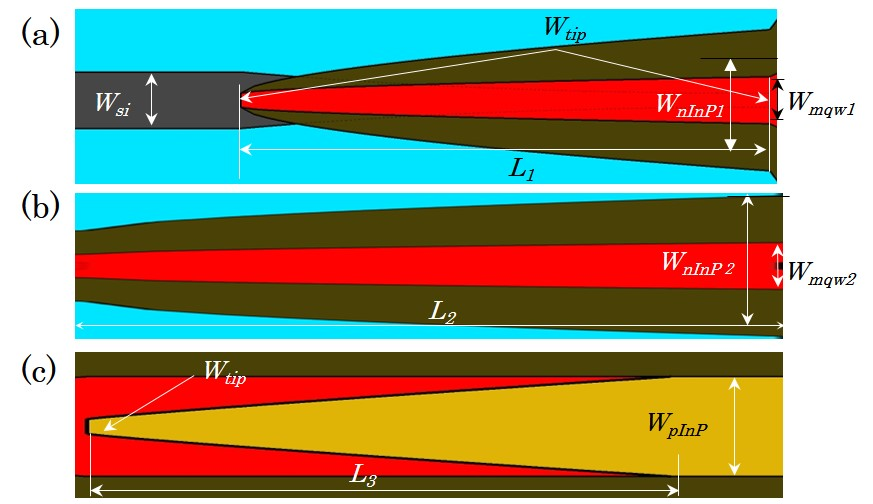
\includegraphics[width=12cm]{./Pictures/fig_ch3_detail_structure.jpg}
	\caption{三段式波导详细的结构参数:(a) 第一段垂直耦合结构;(b)第二段结构;(c)第三段结构}
	\label{fig_ch3_detail_structure}
\end{figure}

\begin{figure}[htb]
	\centering
	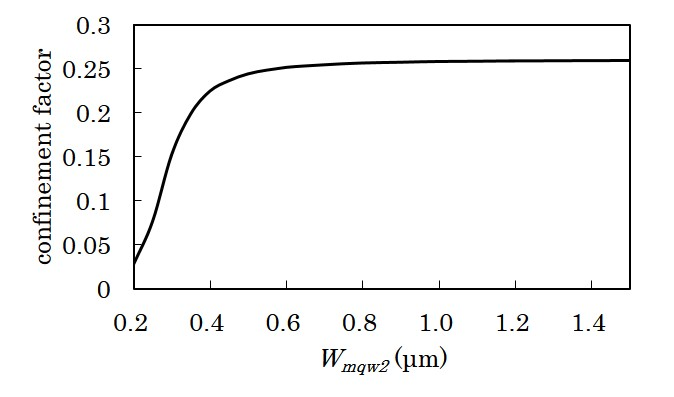
\includegraphics[width=12cm]{./Pictures/fig_ch3_confinement.jpg}
	\caption{光在100 nm厚量子阱区域的限制因子}
	\label{fig_ch3_confinement}
\end{figure}

在每段锥形结构的轮廓我们采用文献[\citenum{sun2009adiabaticity}]中的多项式进行描述\ref{Equ:exponential}:
\begin{equation}
\label{Equ:exponential}
W(x) = w_0+(w_1+w_0)\left(x/L_t\right)^\alpha
\end{equation}
其中,$W(x)$是$x$处的宽度,$w_0$是初始宽度,$w_1$是末尾宽度,$L_t$是锥形结构的长度,$\alpha$是指数项用于定义锥形结构的外形。由于实际工艺中,SCH层和MQW层的材料不能选择性腐蚀,因此他们的形状在此设计中是相同的。为了简化设计,MQW层和n-contact层的指数项$\alpha$保持相同。

在第一段锥形结构中,我们首先选择MQW层锥形结构末端的宽度。从图\ref{fig_ch3_multimode}(b),我们可以看到,当MQW的宽度为$0.5 ~ \mu m$时,基模的等效折射率和高阶模式的等效折射率差别最大,因此我们将其设置为$0.5 ~ \mu m$。由于很薄的n-contact层对模式的影响很小。在这个例子中,我们将n-contact锥形结构末端的宽度设置为$1.5 \mu m$。除此,在第一段锥形结构中,还有3个参数需要设计优化,即锥形结构的长度$L_1$,定义硅锥形结构外形的指数项$\alpha_{si}$和定义III-V锥形结构外形的指数项$\alpha_1$。

在第二段锥形结构中,MQW层末端的宽度与最后硅基混合集成III-V波导的宽度相同,即$W_{mqw2} = 1~\mu m$。我们将n-contact锥形结构的末端设置为$3~\mu m$。除此之外,还有两个参数需要优化,即锥形结构的长度$L_2$以及III-V锥形结构外形的指数项$\alpha_2$。

在第三段锥形结构中,MQW层波导的宽度不变为$1~\mu m$,而p-cladding锥形结构末尾宽度也为$1~\mu m$。而锥形结构的长度$L_3$和p-cladding锥形外形的指数项$\alpha_3$,这两个参数需要进一步优化。

我们采用三维的时域有限差分方法(3D Finite-Difference Time domain method, 3D-FDTD)软件去仿真各段锥形结构的耦合效率\cite{fdtdsolution}。通过分别优化每段的结构参数,实现最高的基模耦合效率。然后,将优化的每段结构在组合成整体结构。一般采用DVS-BCB键合的厚度$h_{BCB}$可以达到30 nm至100 nm。在此,我们选择$h_{BCB} = 50~nm$。之前各段锥形结构中待优化的参数,我们通过扫描,仿真结果见图\ref{fig_ch3_sweep_structure}。我们可以看到硅锥形结构的指数项$\alpha_{si}$对耦合效果没有明显影响。然而,其他的指数项$\alpha_1$,$\alpha_2$,$\alpha_3$对耦合效率有明显的影响。根据图\ref{fig_ch3_sweep_structure}(a)-\ref{fig_ch3_sweep_structure}(c),我们选取$\alpha_{si} = 2.2$,$\alpha_1 = 0.6$,$\alpha_2 = 0.6$,$ \alpha_3 = 0.9$。在扫描指数项时,锥形结构必须有足够的长度。接下来,在确定最佳锥形结构外形时,我们扫描锥形结构的长度。从图\ref{fig_ch3_sweep_structure}(d)到图\ref{fig_ch3_sweep_structure}(f),我们可以看到,当$L_1 = 4~ \mu m$, $L_2 = 1~\mu m$,$ L_3 =  3~\mu m $时,耦合效率已经达到96\%以上,继续增加长度,耦合效率只有3\%的波动。这保证了每段锥形结构都是绝热的。因此,整体锥形结构的长度只$有8 \mu m$。

\begin{figure}[htb]
	\centering
	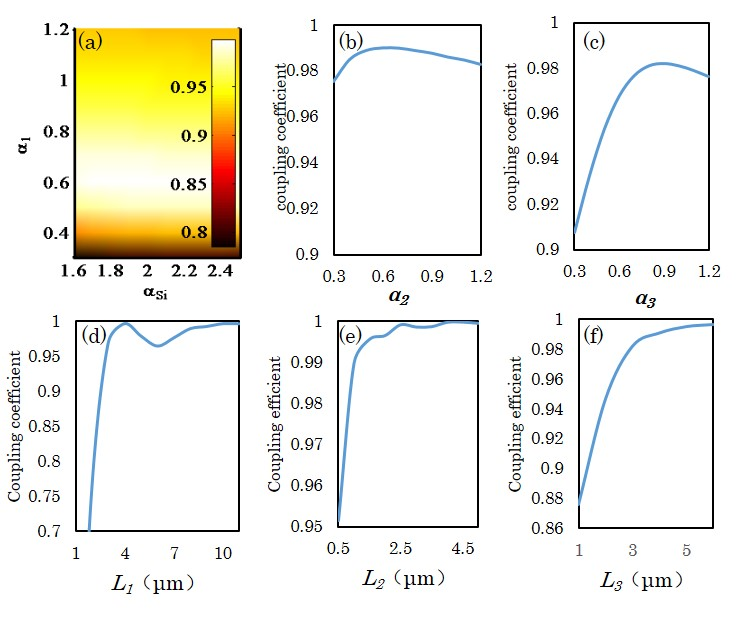
\includegraphics[width=14cm]{./Pictures/fig_ch3_sweep_structure.jpg}
	\caption{各段锥形耦合结构在不同结构参数下的耦合效率:(a)当第一段的锥形结构的长度$L_1 = 4~\mu m$;(b)当第二段的锥形结构的长度$L_2 = 4~\mu m$;(c)当第三段的锥形结构的长度$L_1 = 3~\mu m$;(d)当第一段的锥形结构中$\alpha_{si}= 2.2$,$\alpha_1 = 0.6$;(e)当第一段的锥形结构中$\alpha_2 = 0.6$;(f)当第三段的锥形结构中$\alpha_1 = 0.9$。}
	\label{fig_ch3_sweep_structure}
\end{figure}

图\ref{fig_ch3_8um_taper}展示了三段式锥形结构的仿真结果。从图\ref{fig_ch3_8um_taper}(a)可以看到,当基模的耦合效率达到95\%上时,对应的波长带宽达到了100 nm。 当基模的耦合效率达到90\%上时,对应的波长带宽达到了300 nm。从图\ref{fig_ch3_8um_taper}(a)也可以看出,在短波长,第一段锥形结的损耗构限制了耦合效率。在长波长,却是第三段锥形结构的损耗限制了耦合效率。在图\ref{fig_ch3_8um_taper}(b),我们分析了不同$h_{BCB}$下,耦合效率的变化。可以看到$8 ~\mu m$长的锥形结构在$h_{BCB}$从20 nm变化到80 nm时,耦合效率依旧保持在90\%以上。图\ref{fig_ch3_8um_taper}(c)展示了在工作波长$1.55~\mu m$,$h_{BCB} =  50 ~nm$时,光场从硅波导耦合到硅基混合集成III-V波导的模式耦合图。可以看到,光在两个波导之间的相互耦合主要发生在第一段锥形结构。因此,第一段锥形结构对$h_{BCB}$的变化十分敏感。当光耦合到III-V后,$h_{BCB}$的变化就几乎不会影响光场的变化,因此第二段和第三段锥形结构几乎不影响锥形结构的耦合效率。而在图\ref{fig_ch3_8um_taper}(b)中,也展示了$h_{BCB}$的变化对第一段锥形结构的耦合效率影响最大。

\begin{figure}[htb]
	\centering
	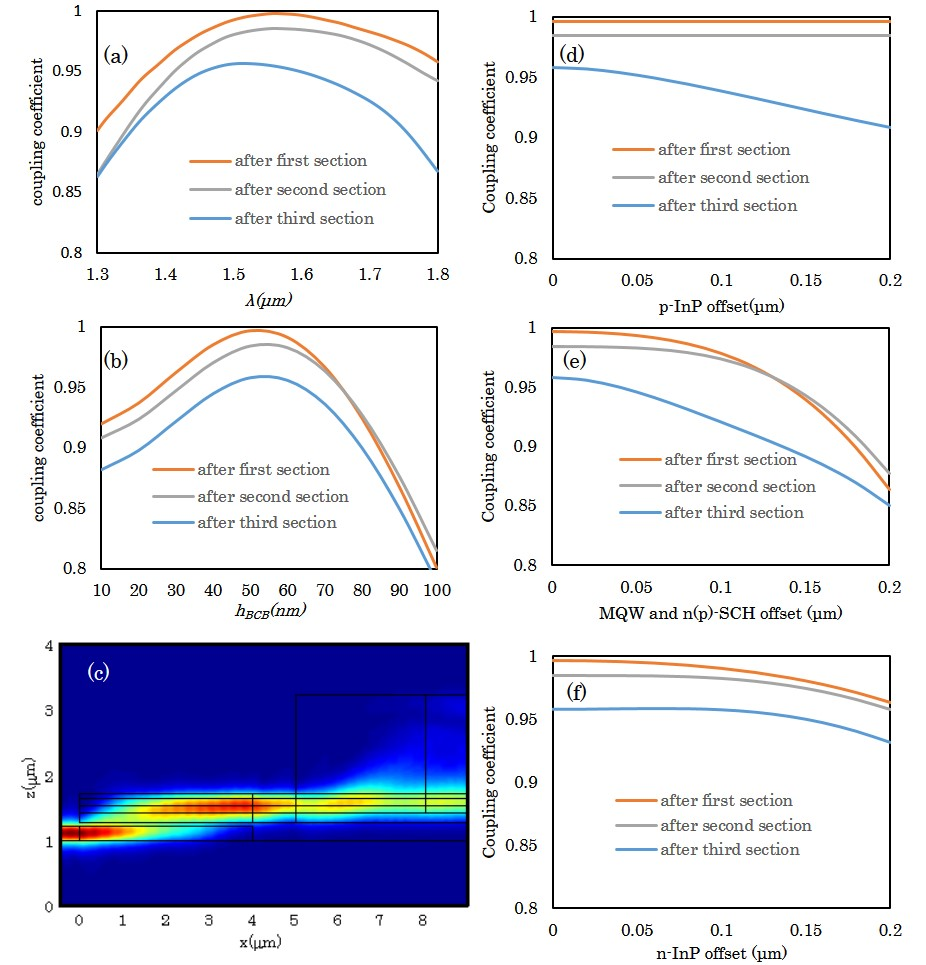
\includegraphics[width=14cm]{./Pictures/fig_ch3_8um_taper.jpg}
	\caption{$8~\mu m$耦合结构的性能:(a)当$h_{BCB}=50~nm$时,波长变化对耦合效率的影响;(b)当工作波长为$1550~nm$时,$h_{BCB}$变化的影响;(c)当工作波长为$1550~nm$,$h_{BCB}=50~nm$时,模场在耦合结构中的传播图;(d)当p-cladding层出现套刻误差的影响;(e)当MQW层和SCH层出现套刻误差的影响;(f)当n-contact层出现套刻误差的影响。}
	\label{fig_ch3_8um_taper}
\end{figure}

加工这三段式的耦合结构需要三次掩膜版的套刻工艺。它们分别用于定义p-cladding层,MQW层和SCH层,以及n-contact层。因此,我们进一步分析了掩膜版套刻偏离对耦合效率的影响。从图\ref{fig_ch3_8um_taper}(d)可以看到,p-cladding层的套刻偏离只会影响第三段锥形结构的耦合效率。这是由于p-cladding只存在于第三段锥形耦合结构中。从图\ref{fig_ch3_8um_taper}(e)可以看出,MQW层和SCH层的套刻偏离对第一段和最后一段耦合结构的耦合效率有明显的影响,并且MQW层和SCH层的套刻偏差是对整体耦合结构效率的影响最大的。从图\ref{fig_ch3_8um_taper}(f)可以看出,n-contact层的套刻偏差对整体耦合效率只有微弱的影响。基于以上的分析,为了使$8 \mu m$长的耦合结构保持90\%以上的耦合效率,MQW层和SCH层的套刻精度需要保持在100~nm的范围内。

为了增加耦合结构的光学带宽,对$h_{BCB}$变化的容忍度和对掩膜套刻精度的容忍度,第一段和最后一段耦合结构的耦合效率需要提高。其中一个简单的方式是通过增加耦合结构的长度。我们将$L_1$增加到了$8~\mu m$,并且将$L_3$增加到了$5~\mu m$,并且保持其他的参数不变。整个耦合结构的长度增加到了$14~\mu m$。这个增长的锥形耦合结构的仿真结果如图\ref{fig_ch3_14um_taper}所示。

从图\ref{fig_ch3_14um_taper}(a)可以看出,这个增长耦合结构的模式耦合效率在95\%以上,对应的波长范围达到了200 nm。在90\%以上耦合效率的波长范围达到了500 nm。从图\ref{fig_ch3_14um_taper}(b)可以看到,当$h_{BCB}$从0 nm变化到100 nm时,整个耦合结构的耦合效率依旧能保持在95\%以上。图\ref{fig_ch3_14um_taper}(c)展示了当工作波长为$1.55 ~\mu m, h_{BCB} = 50~nm$时,在这$14~\mu m$长耦合结构的模场传播图。

从图\ref{fig_ch3_14um_taper}(d)到图\ref{fig_ch3_14um_taper}(f)展示了每层掩膜版套刻误差对这个$14~\mu m$长锥形结构的耦合效率的影响。通过与之前图\ref{fig_ch3_8um_taper}(d)至图\ref{fig_ch3_8um_taper}(f)的比较,我们可以看到长度增加的锥形结构对工艺中套刻误差的容忍度更高。当p-cladding层的套刻误差在$\pm 200~nm$的范围内,当MQW层和SCH层的套刻误差在$\pm 100~nm$的范围内,当n-contact层的套刻误差在$\pm 150~nm$的范围内时,整个锥形结构的耦合效率依旧能保持在95\%以上。通过之前的讨论分析,我们可以发现第二段锥形结构中MQW层和SCH层掩膜的套刻精度对整个锥形结构的偶耦合效率影响最大。

\begin{figure}[htb]
	\centering
	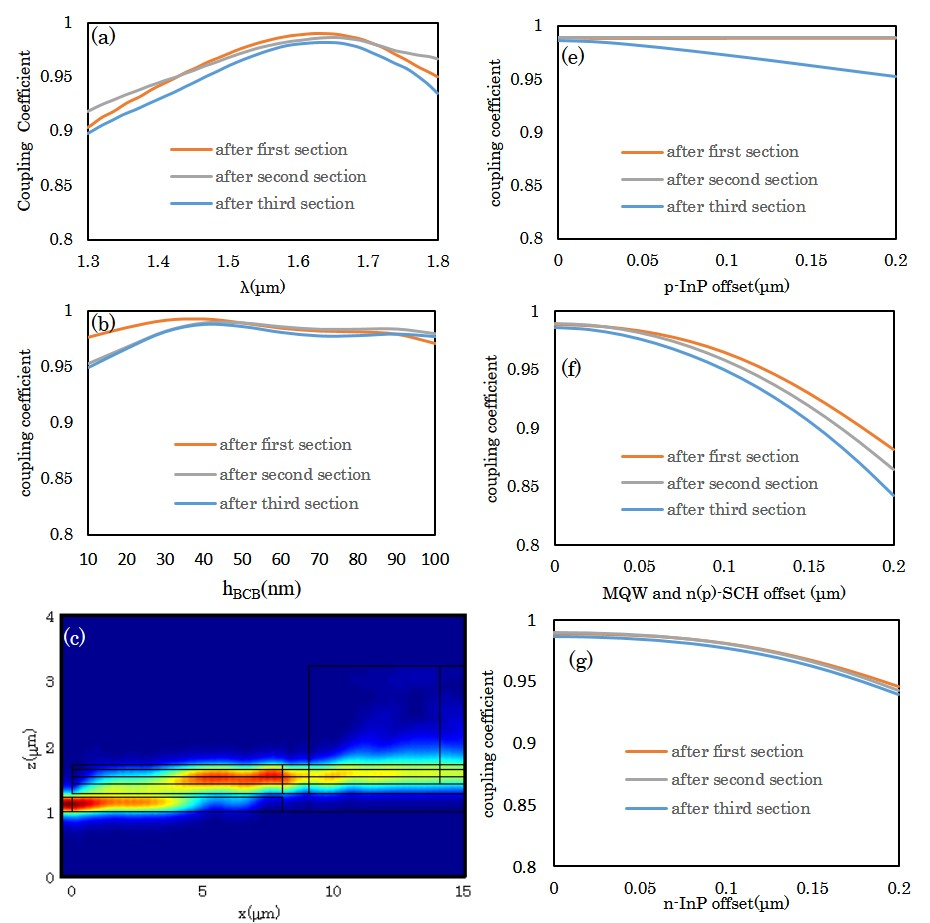
\includegraphics[width=14cm]{./Pictures/fig_ch3_14um_taper.jpg}
	\caption{$14~\mu m$长耦合结构的性能:(a)当$h_{BCB}=50~nm$时,波长变化对耦合效率的影响;(b)当工作波长为$1550~nm$时,$h_{BCB}$变化的影响;(c)当工作波长为$1550~nm$,$h_{BCB}=50~nm$时,模场在耦合结构中的传播图;(d)当p-cladding层出现套刻误差的影响;(e)当MQW层和SCH层出现套刻误差的影响;(f)当n-contact层出现套刻误差的影响。}
	\label{fig_ch3_14um_taper}
\end{figure}

通常而言,硅基混合III-V平台中的调制器相比激光器和放大器,不需要高的耦合效率。因此,$8~\mu m$长的耦合结构非常适合硅基光调制器。而对于激光器和光放大器,由于三段式后结构的第一段没有p-cladding层,所以无法进行有效的电泵浦。又因为激光器和光放大器的MQW的吸收峰就落在其激光出射的波段,因此第一段耦合结构可能带来比较大的损耗。而对于电吸收光调制器,在没有电压下的MQW的吸收峰是小于工作波长的,因此就没有这个问题。文献[\citenum{tang201150,tang2012energy,tang2012over}]中特意用离子注入对锥形耦合结构进行电学隔离,而在我们所提出的三段式耦合结构中,我们通过在一段锥形结构中去除了p-cladding层,自然而然地进行了电学的隔离。

\section{紧凑三段式耦合结构的工艺探索}
紧凑型三段式耦合结构可以用于硅基混合集成III-V平台下使用矩形波导结构的电吸收光调制器。根据上章分析,这种调制器具有调制带宽大的特点。而目前硅基混合集成III-V的电吸收光调制器都是蘑菇型波导,由于其波导宽度大于$1~\mu m$,定义波导图形是采用接触式光刻。而在矩形波导的光调制器以及三段式耦合结构中,波导宽度都需要小于$1~\mu m$。因此,这种结构无法用现有的接触式光刻制作。

在此我们首次尝试用电子束光刻制作三段式耦合结构。虽然电子束光刻已经在实验室中被广泛用于制作纯硅光器件,但是没有被用于制作硅基混合集成III-V波导。其中两个主要原因是,电子束的光刻胶的厚度比较薄,和电子束容易被散射的问题。如图\ref{fig_ch3_ele_sca}(a),如果片子表面的局部高度起伏大于光刻胶的厚度,那么将会严重影响光刻胶的表面的平整度,从而影响定义图形的精确尺寸。图\ref{fig_ch3_ele_sca}(b)展示了在一个陡直的侧壁附近套刻图形,那么电子束就会被侧壁散射,从而使图形展宽。
\begin{figure}[htb]
	\centering
	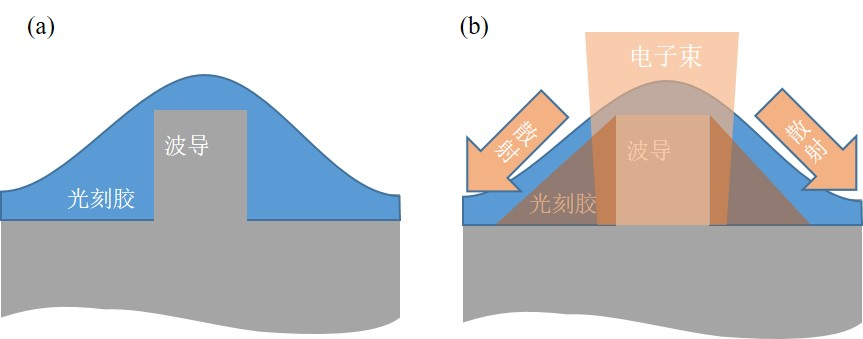
\includegraphics[width=12cm]{./Pictures/fig_ch3_ele_sca.jpg}
	\caption{(a)片子局部表面起伏太大,导致光刻胶匀完后表面不平整;(b)陡直侧壁处套刻图形,导致电子被散射,使曝光图形展宽。}
	\label{fig_ch3_ele_sca}
\end{figure}

电子束胶的厚度普遍小于1~$\mu m$,适合用于套刻和定义波导高度差普遍小于500~nm的纯硅光器件图形。然而在硅基混合集成III-V平台上,波导的高度差会达到2~$\mu m$。尤其在制作三段式耦合结构中,套刻第二层锥形结构时,需要在高度1.5~$\mu m$的p-cladding上再精确地套刻MQW层和SCH层的图形。这将会遇到定义图形展宽,变形的问题。下面将详细介绍工艺步骤解决这两个问题。

第一步定义p-cladding层图形,如图\ref{fig_ch3_step1_2}(a)所示。我们首先在混合集成的III-V外延片上用等离子体增强化学气相沉积(Plasma Induced Chemical Vapor Deposition,PECVD)生长一层300~nm-400~nm厚的二氧化硅(SiO\SB{2})。在生长之前,需要将片子在温度100摄氏度以上的热盘上,放置3min,使表面和背面的水汽蒸发,以防片子放入PECVD,片子滑动。在匀电子束胶之前,SiO\SB{2}表面需要用增粘剂处理,使其与ma-N 2403的粘附性增强。我们是将长完二氧化硅的片子,用甲烷轰击,以提高其和ma-N 2403的粘附性。然后,再匀电子光刻胶ma-N 2403\cite{man2403}。这是一种负胶,厚度大概300 nm左右。紧接着,我们将其放到90摄氏度的热盘上90 s。做完这步,就意味着我们的片子已经准备好放入电子束光刻机中曝光了。根据图形的最小尺寸和胶的特性,选用相应的电场强度和孔径的电子枪,从而使图形写的时间短并且精度满足要求。我们使用电场强度为30~KV,孔径为20~$\mu m$的电子枪。除此之外,不同图形的面积,形状,需要不同的曝光计量,和电子束移动的方式。这个需要根据不同材料,不同光刻胶,调整。我们写完图形后,用显影液ma-D525显影2分30秒。最后为了使光刻胶侧壁光滑些,我们将其放入110摄氏度的烘箱中,将光刻胶进行回流,从而减小光刻胶侧壁的粗糙度。

第二步将光刻胶的图形转移到p-cladding层,如图\ref{fig_ch3_step1_2}(b)所示。定义好光刻图形后,我们将片子背面涂上导热胶,放到感应耦合等离子体刻蚀机(Inductively Coupled Plasma, ICP)中,利用CH\SB{3} : CF\SB{4} = 50 : 6的混合气体,在3~mT的压强,在适当的射频功率下,进行刻蚀。刻蚀结束后,由于光刻胶已经被碳化,无法用丙酮去除干净。在此,我们用强力去胶剂(N-甲基吡咯烷酮)将残留的光刻胶去除干净,再把片子放入利用氧等离子体的去胶机中,将残留的光刻胶彻底取出干净。此时,图形已经转移到二氧化硅上。接下来,我们ICP刻蚀p-contact(材料为InGaAs) 层和p-cladding(材料为InP)层。此时ICP的中的混合气体是H\SB{2}:Cl\SB{2}:CH\SB{4}:Ar = 5:7:10:5,腔内温度为60摄氏度,压强为4~mT。由于ICP不是选择性刻蚀,会同时刻蚀SCH和p-cladding层。为此,我们根据刻蚀速率,当InP还剩下100-300 nm时,换成湿法腐蚀。我们采用HCl:H\SB{2}O = 1:1的溶液在20摄氏度下腐蚀InP。此时的腐蚀速率大概100~nm/min。腐蚀后,在显微镜下观察片子表面颜色是否均匀,表面是否光滑。此时在波导外,片子的上表面是SCH层。最后,我们将片子放入BOE (Buffered Oxide Etch,HF:NH\SB{4}F=1:6)的溶液中,去除二氧化硅掩膜。实际片子的腐蚀电镜图见图\ref{fig_ch3_step1_2}(c)。

\begin{figure}[htb]
	\centering
	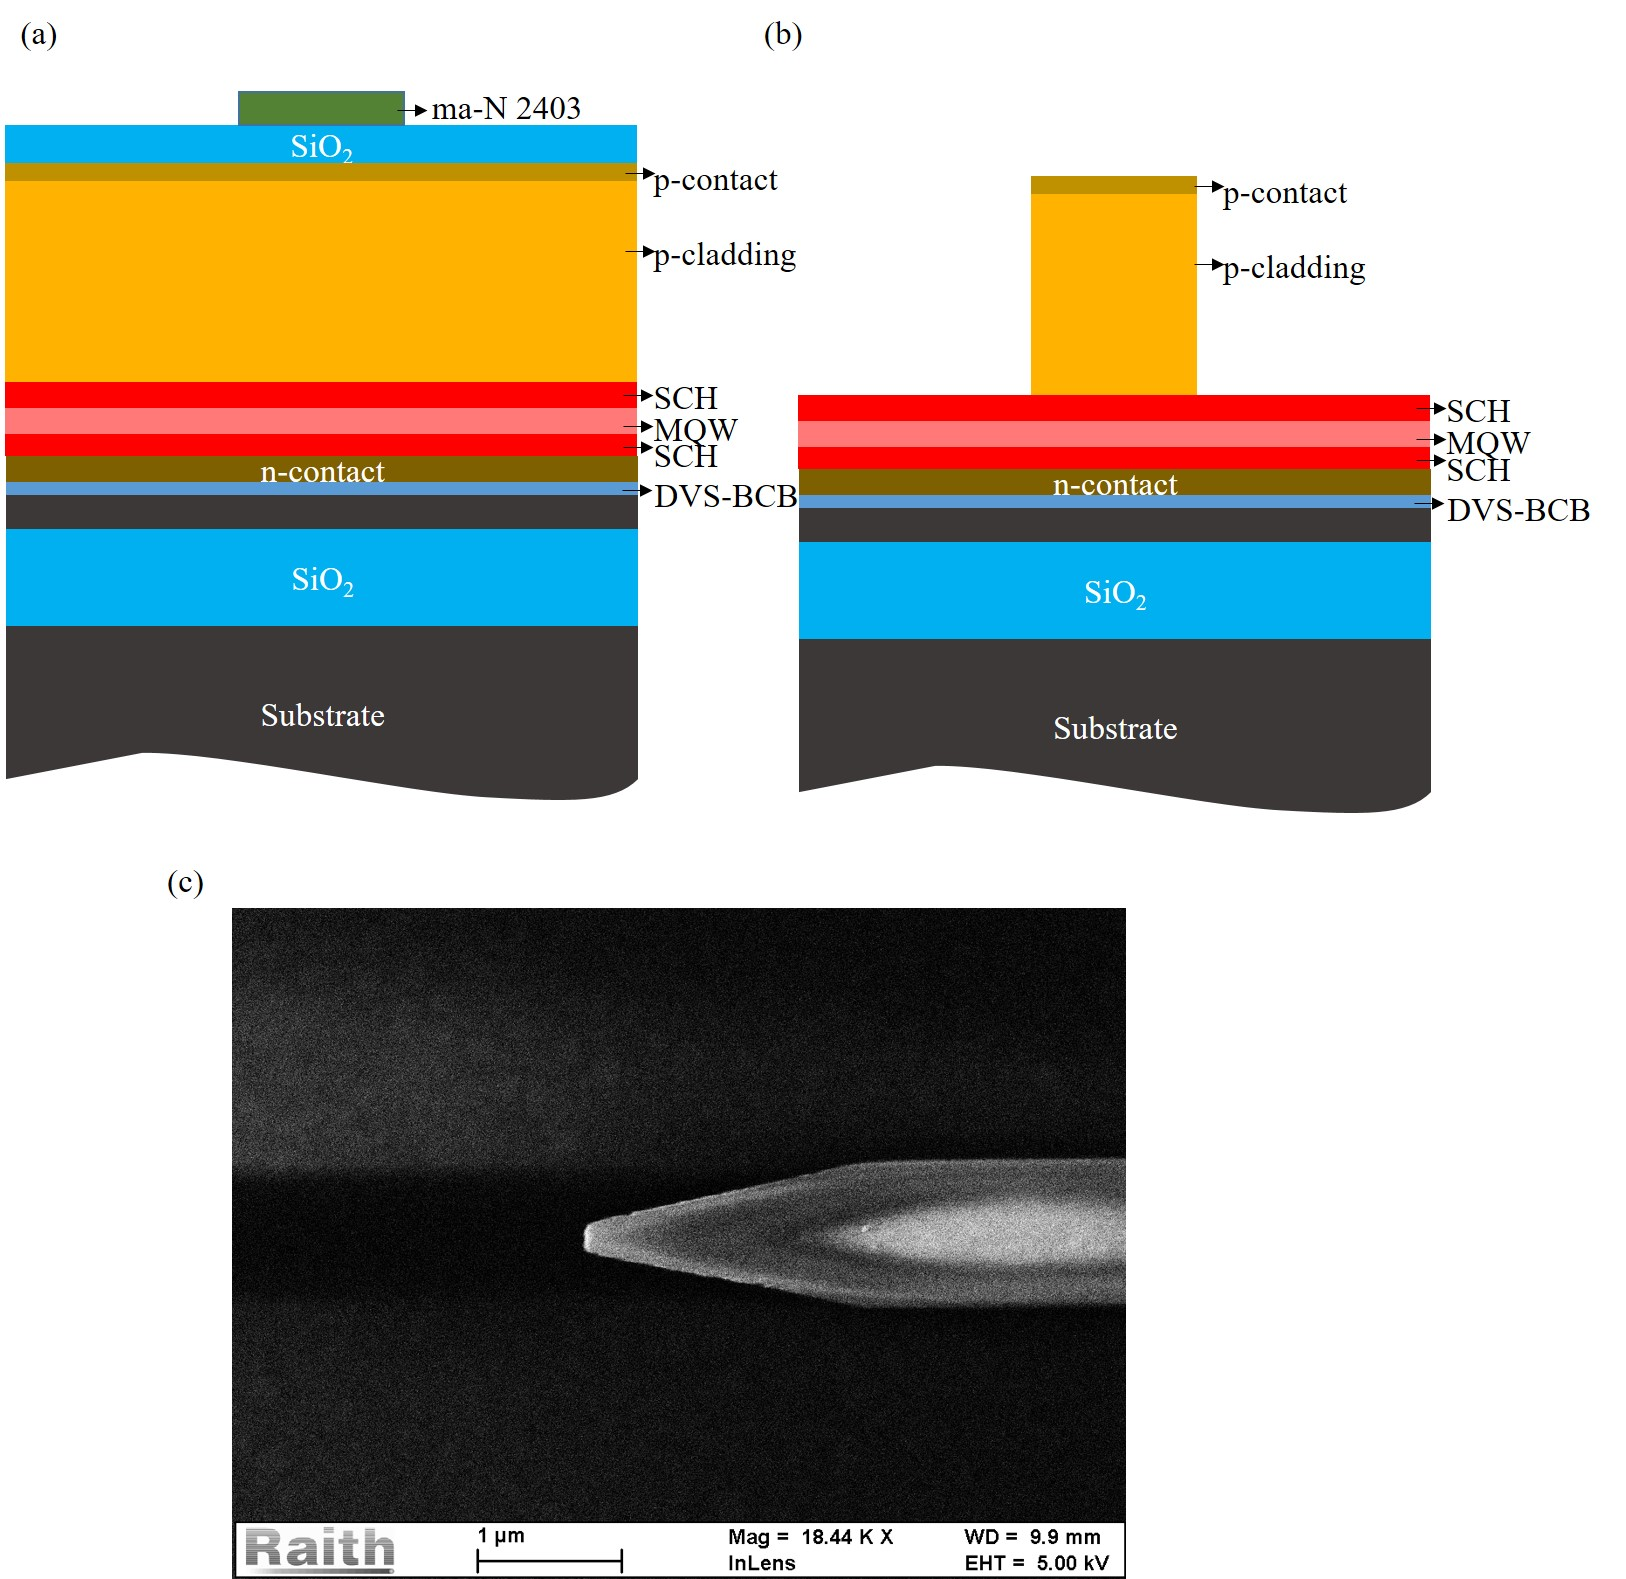
\includegraphics[width=14cm]{./Pictures/fig_ch3_step1_2.jpg}
	\caption{(a)第一步结束后的波导截面示意图;(b)第二步结束后的波导截面示意图;(c)第二步结束后器件的电镜俯视图}
	\label{fig_ch3_step1_2}
\end{figure}

第三步套刻MQW层和SCH层的图形,如图\ref{fig_ch3_step3_4}(a)所示。接下来,我们需要再利用PECVD沉积一层300nm左右的二氧化硅。从图\ref{fig_ch3_step3_4}(b)可以看到沉积的二氧化硅也会把波导的侧壁包裹住。接下来,与步骤一的匀胶过程一样,对SiO\SB{2}进行表面处理提高其对光刻胶的粘附性。在此我们使用正胶ZEP~520套刻图形\cite{ZEP520},而不是负胶。如果使用负胶的话,定义图形时,就会出现之前所述的电子被波导的侧壁散射的问题,如图\ref{fig_ch3_ele_sca}(b)所示。实际中被电子散射展宽的波导如图\ref{fig_ch3_step3_4}(c)所示。而采用正胶时,电子束写图形外侧的光刻胶,避免了与波导侧壁的接触,从而可以在波导附近套刻出精准的图形。我们将图形定义的宽度稍微比实际的宽度偏大500~nm左右,通过下一步的湿法腐蚀,将这个宽度余量弥补回来。旋涂完ZEP胶,我们将其放在180摄氏度的热板上10分钟。至此片子可以放入电子束光刻机中写图形了。我们使用电场强度为30~KV,孔径为20~$\mu m$的电子枪套刻图形。套刻完图形后,我们将其放到显影液中显影,然后进行定影。最后,提高光刻胶与二氧化硅的刻蚀比,我们其放到60到120摄氏度的缓慢升温的热盘上10分钟,对光刻胶硬化。

第四步将光刻胶的图形转移到MQW层和SCH层,如图\ref{fig_ch3_step3_4}(d)所示。首先与第二步相同,ICP刻蚀SiO\SB{2}。然后,然后利用强力去胶剂和氧等离子体的去胶机,将残留的光刻胶彻底去除干净。接下来,就是将图形从SiO\SB{2}上转移到MQW层和SCH层。由于MQW和SCH的成分是InAlGaAs,因此我们使用柠檬酸(citric) : H\SB{2}O\SB{2} = 20 : 1的溶液,在室温下进行腐蚀。每隔5分钟测量腐蚀深度,确定腐蚀速率。我们适当过腐蚀,进行内刻蚀(undercut)将波导宽度缩小到设计值。最后,我们将片子放入BOE溶液中,去除二氧化硅掩膜。此时的波导如图,如图\ref{fig_ch3_step3_4}(e)所示。

\begin{figure}[htb]
	\centering
	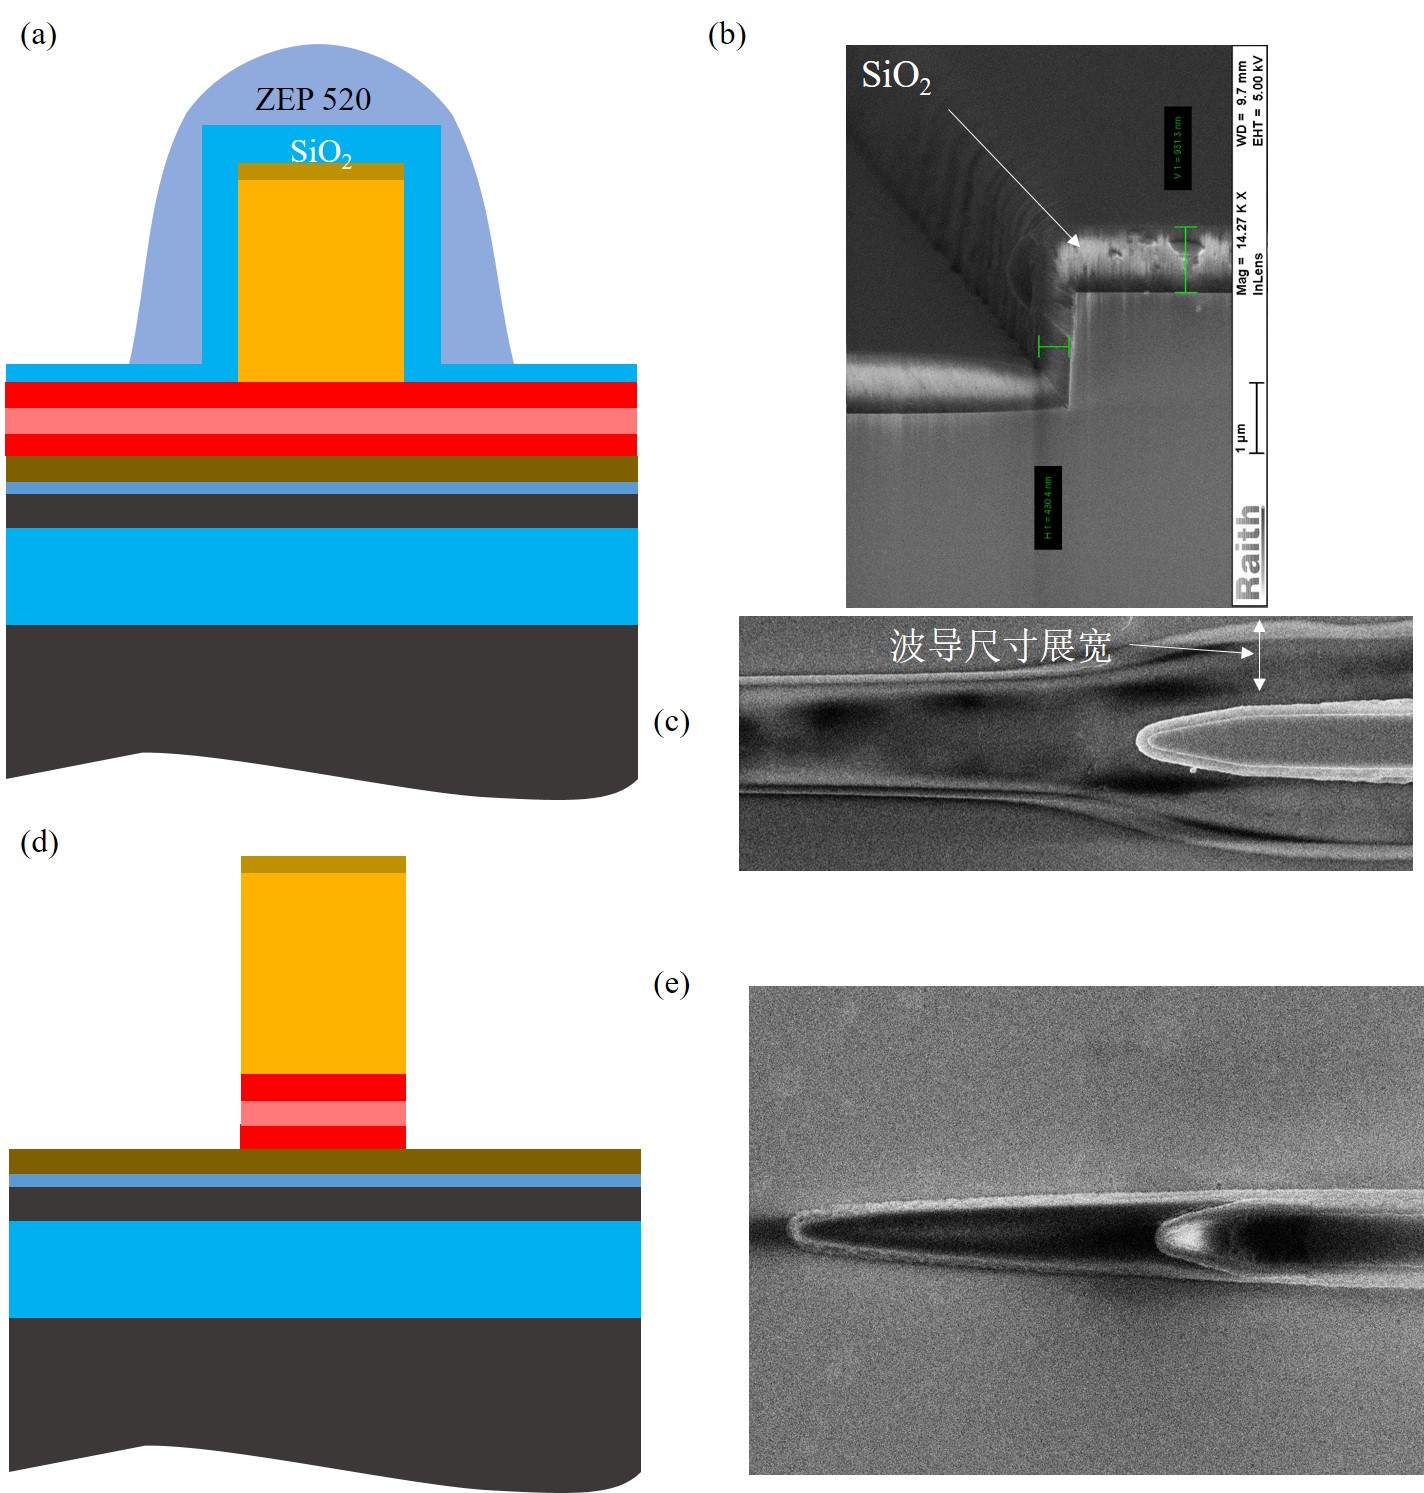
\includegraphics[width=14cm]{./Pictures/fig_ch3_step3_4.jpg}
	\caption{(a)第三步结束后的波导截面示意图;(b)二氧化硅包裹着的波导截面电镜图;(c)用负胶导致套刻图形,导致展宽的电镜图;(d)第四步结束后的波导截面示意图;(e)第四步结束后的器件电镜俯视图。}
	\label{fig_ch3_step3_4}
\end{figure}


第五步套刻n-contact层的图形,如图\ref{fig_ch3_step5_6}(a)所示。与第三步相同,首先利用PECVD沉积一层300 nm左右的二氧化硅膜。再对SiO\SB{2}表面处理提高其对光刻胶的粘附性。我们在此也使用正胶ZEP 520套刻图形。旋涂完ZEP胶,前烘180摄氏度的热板上10分钟。接下来电子束光刻机配置电场强度为30~KV,孔径为20~$\mu m$的电子枪,套刻图形。结束后放到显影液中显影,然后进行定影。最后,后烘片子,将其放置在60到120摄氏度缓慢升温的热盘上10分钟,提高光刻胶与二氧化硅的刻蚀比。

第六步将光刻胶的图形转移到n-contact层,如图\ref{fig_ch3_step5_6}(b)所示。与第二步相同,ICP刻蚀SiO\SB{2}。然后利用强力去胶剂和氧等离子体的去胶机,将残留的光刻胶彻底去除干净。接下来,将片子放入ICP进行刻蚀。n-contact层也是InP,因此配方与第二步中描述的一样。刻蚀完InP后,,我们将片子放入BOE溶液中,去除二氧化硅掩膜。至此,使用电子束光刻制作三段式耦合结构已经完成,如图\ref{fig_ch3_step5_6}(c)所示。由于ICP可是InP的洁净度要求很高,最好单个ICP刻蚀两三种材料相似的材料,否则会把ICP墙体弄脏。如果腔体肮脏的话,可能会很难清洗,就会使刻蚀完的结构产生如图\ref{fig_ch3_step5_6}(c)所示的小的脏颗粒。
\begin{figure}[htb]
	\centering
	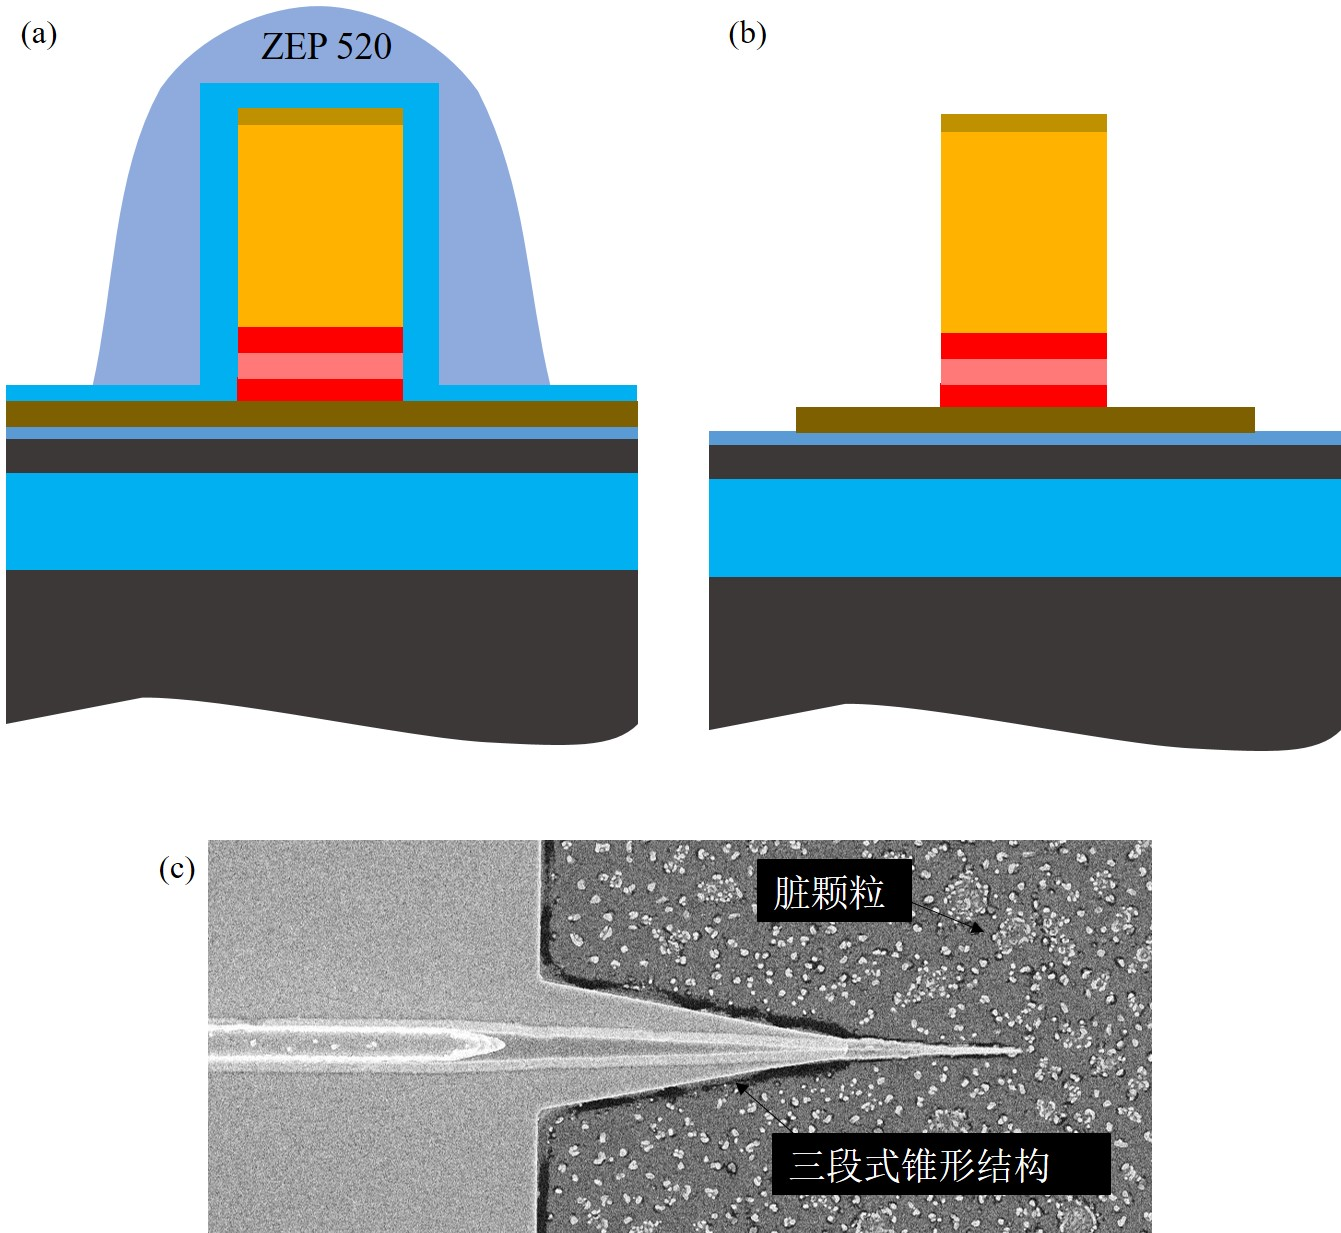
\includegraphics[width=14cm]{./Pictures/fig_ch3_step5_6.jpg}
	\caption{(a)第五步结束后的波导截面示意图;(b)第六步结束后的波导截面示意图;(c)第六步结束后的器件电镜俯视图。}
	\label{fig_ch3_step5_6}
\end{figure}

\section{本章小结}
在本章中,我们解决硅基混合平台中硅波导和混合集成III-V波导的耦合问题。并且我们分析了限制硅波导和混合集成III-V波导耦合器件长度的原因,是来自于III-V波导的高阶模式容易在光耦合的过程中被激发出来。为此,我们设计了三段式锥形耦合结构,实现了长度只有$8 ~\mu m$的耦合结构。这是目前最小的耦合结构,并且基模的耦合效率达到95\%,对应的工作波长带宽达到100~nm。这种结构能增加硅基混合集成III-V器件的集成度。除此之外,考虑到实际工艺问题,我们进一步分析了制作过程中,套刻精度和硅与III-V键合层厚度的对耦合效率的影响。我们发现MQW层和SCH层的套刻精度对波导的耦合效率影响最为明显。最后,我们首次探索利用电子束光刻定义和套刻这种三段式锥形结构的工艺流程。通过巧妙地利用正胶,曝光的胶保留下来的性质,解决了利用电子束在高度落差大的波导附近套刻,出现由电子被波导侧壁反射而导致的线形展宽的问题。最后,我们初步实现了利用电子束光刻机在硅基混合集成III-V平台上制作了三段式锥形耦合的结构。